
\fitter is an open source code and it can be downloaded from the dedicated webpage \cite{herafitter:page}
together with its supporting documentation and 
% A README file is provided within the package together with the 
fast grid theory files (described in section \ref{sec:techniques}) associated with the properly formatted data files available in \fitter.
The source code contains all the relevant information to perform QCD fits with HERA DIS data as a default 
set~\footnote{Default settings in \fitter are tuned to reproduce the central HERAPDF1.0 set.}. 
The performance time depends on the fitting options and varies from 10 minutes 
(using 'FAST' techniques as described in section \ref{sec:techniques}) to several hours when full uncertainties are estimated. The \fitter code is a combination of \tt C++ \rm and \tt Fortran 77\rm libraries with minimal 
dependencies, i.e. for the default fitting options no external dependences are required except \qcdnum evolution program \cite{qcdnum} and CERN libraries. 
The \tt ROOT \rm  libaries are only required for the drawing tools and when invoking \applgrid.  
Drawing tool inbuilt in \fitter provides a qualitative and quantitative assessment of the results.
Fig.~\ref{fig:data} shows an illustration of a comparison between the inclusive NC data from the HERA I
with the predictions based on 
HERAPDF1.0 PDFs.
The consistency of the measurements and the theory is expressed by pulls, defined as a difference between data and theory divided by the uncorrelated error of the data. 
In each kinematic bin of the measurement, pulls are provided in units of standard deviation (sigma).  
%As an additional consistency check between data and the theory predictions, pull information, defined as the difference between data and prediction divided by the uncorrelated uncertainty of the data, is displayed in units of sigma shifts for each given data bin.
\begin{figure}[!ht]
   \centering
   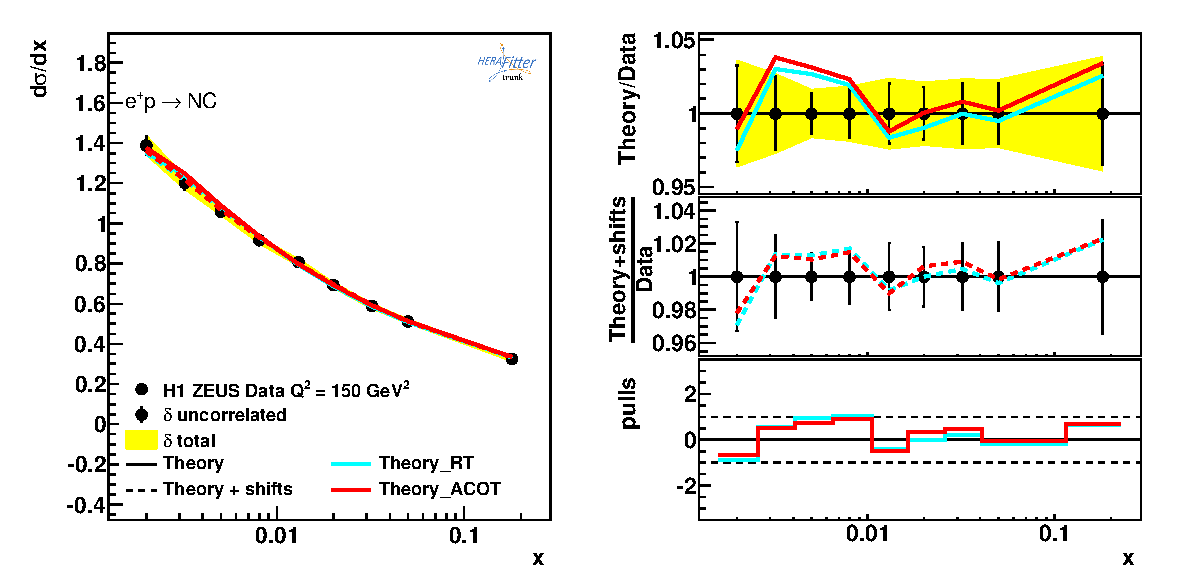
\includegraphics[width=8.6cm]{datatheory.pdf}
   \caption{An illustration of the consistency of HERA measurements~\cite{h1zeus:2009wt} and the theory predictions, 
       obtained in \fitter with the default drawing tool.} 
       %In addition, ratio plots are also provided together with the pull distribution (right panel).}    
 \label{fig:data}
\end{figure}

%\end{description}
%
In \fitter there are also cache options, fast evolution kernels, and usage of the OpenMP (Open Multi-Processing) 
interface which allows parallel applications of the GM-VFNS theory predictions in DIS. 
In addition, the \fitter references and GNU public licence are provided 
together with the main source code. 


